\documentclass[a4paper,11pt]{amsart}

\usepackage{mathrsfs}
\usepackage{gensymb}
\usepackage{circuitikz}
\usepackage{tikz}
\usetikzlibrary{arrows.meta}
\usepackage{caption}
%\usepackage{newtxmath}
%\usepackage{txfonts}
\usepackage{times}
\usepackage[top=27mm, left=23mm, bottom=23mm, right=23mm]{geometry}
\usepackage{amsfonts, amssymb, amsgen, amsthm, amscd, amsmath}
\usepackage{mathtools}
\mathtoolsset{showonlyrefs=true}
%\usepackage{pxfonts}
\usepackage{bm}
%\usepackage{mathpazo}
\usepackage{domitian}
\usepackage[T1]{fontenc}
\usepackage{upgreek}
\let\oldstylenums\oldstyle

\usepackage{enumerate}
\usepackage{color}
\usepackage[all]{xy}

\newtheorem{theorem}{Theorem}[section]
\newtheorem{proposition}[theorem]{Proposition}
\newtheorem{lemma}[theorem]{Lemma}
\newtheorem{corollary}[theorem]{Corollary}
\newtheorem{claim}[theorem]{Claim}
\theoremstyle{definition}
\newtheorem{remark}[theorem]{Remark}
\newtheorem{example}[theorem]{Example}
\newtheorem{definition}[theorem]{Definition}

\newcommand{\outimes}[2]{\overset{#1}{\underset{#2}{\otimes}}}
\newcommand{\C}[1]{\mathcal{#1}}
\newcommand{\B}[1]{\mathbb{#1}}
\newcommand{\G}[1]{\mathfrak{#1}}
\newcommand{\rmod}[1]{\text{{\bf Mod}-}{#1}}

\newcommand{\Span}{\text{\rm Span}}
\newcommand{\Tor}{\text{\rm Tor}}
\newcommand{\Ind}{\text{\rm Ind}}
\newcommand{\Res}{\text{\rm Res}}
\newcommand{\Ext}{\text{\rm Ext}}
\newcommand{\Hom}{\text{\rm Hom}}
\newcommand{\CoInd}{\text{\rm CoInd}}
\newcommand{\Simp}{{\Delta}}
\newcommand{\Diff}{{\Omega}}
\newcommand{\xla}[1]{\xleftarrow{#1}}
\newcommand{\colim}{\text{colim}}
\renewcommand{\baselinestretch}{1.15}
\renewcommand\parallel{\mathrel{/\mskip-2.5mu/}}
\setlength{\parskip}{1.2mm}
\setlength{\parindent}{0mm}

\title{Electromagnetism Assignment For The Forth Time}

\author{Haixuan Lin - 23307110267}
\email{23307110267@m.fudan.edu.cn}


\address{Fudan University, Physics Department, China}

\begin{document}
	
	\begin{abstract}
		Here is the electromagnetism assignment for the forth time which is for the corse given by professor Weichao Liu. In order to practise the expertise in scientific film of physics, students need to practise using \LaTeX to composing their own work, even if this is only a ordinary homework.
	\end{abstract}
	
	\maketitle
	
	\section*{Main Text}
	
	\subsection*{4-1}
	\subsubsection*{(a)}
	The straight part of the wire does not contribute a magnetic field, and the semicircular part contributes half the magnetic field of the circular wire.
	$$
	B_a =  \frac{1}{2}\frac{\mu _0I}{2R}=\frac{\mu _0I}{4R}
	$$
	\subsubsection*{(b)}
	Equal to the field strength generated by the circular wire at the center of the circle.
	
	$$
	B_b = 0
	$$
	\subsubsection*{(c)}
	Is equal to the contribution of the circular wire plus the contribution of the parallel straight wire.
	$$
	B_c= \frac{\mu _0I}{2R}+\frac{\mu _0I}{2\pi}\frac{1}{R}=\frac{\mu _0I}{2\pi R}\left( 1+\pi \right)
	$$
	\subsubsection*{(d)}
	Equal to the contribution of a quarter of a circle.
	$$
    B_d=\frac{\mu _0I}{8\pi R}
	$$
	\subsubsection*{(e)}
	Consider the difference between the contributions of the two wires.
	$$
	B_e=\frac{\mu _0I\theta}{4\pi}\left( \frac{1}{R_2}-\frac{1}{R_1} \right) 
	$$
	\subsubsection*{(f)}
	Consider the sum of the contributions of two semicircles.
	
	$$
	B_f=\frac{\mu _0I}{4}\left( \frac{1}{R_1}+\frac{1}{R_2} \right) 
	$$
	\subsection*{4-6}
	According to Biot-Savart law:
	$$
	B=\frac{\mu _0}{4\pi}\frac{ev}{a_{0}^{2}}=15.4\thinspace\mathrm{T}
	$$
	
	\subsection*{4-15}
	% TODO: \usepackage{graphicx} required
	\begin{figure}
		\centering
		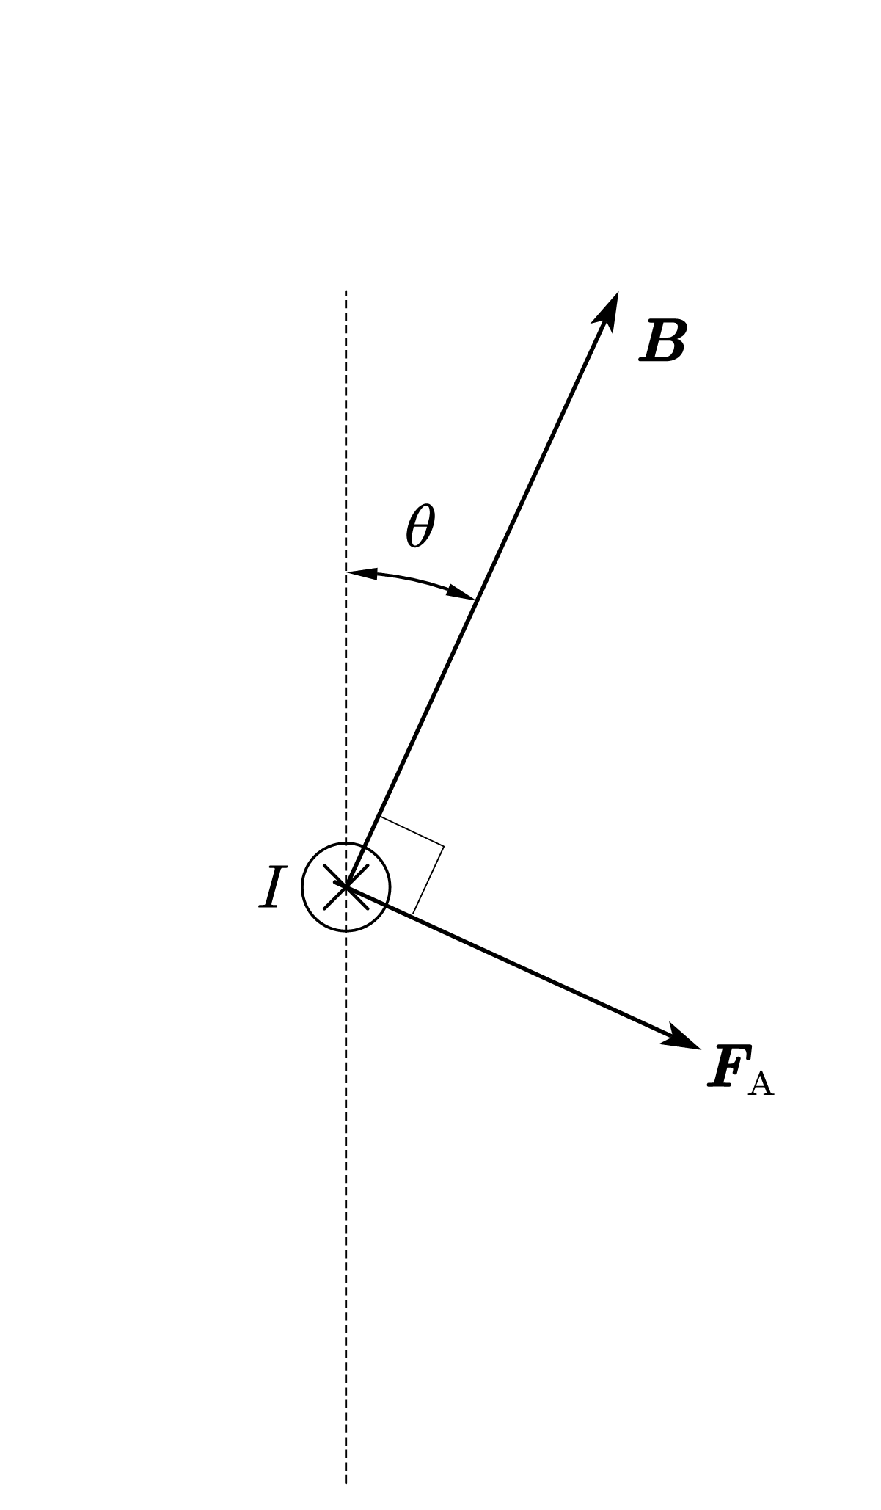
\includegraphics[width=0.3\linewidth]{4-17}
		\caption*{}
		\label{fig:4-17}
	\end{figure}
	As shown in the figure, the radial force components will cancel each other, and the resultant force is downward.
	$$
	F=BIL\sin\theta=2\pi RIB\sin\theta
	$$
	
	\subsection*{4-17}
	Potential energy analysis using magnetic moment and magnetic field.
	$$
	E_p=-a^2IB\cos \theta 
	$$
	And $\theta = <\bm{B}, \bm{S}>.$
	$$
	E=\frac{1}{2}J\dot{\theta}^2-a^2IB\cos \theta =\frac{1}{2}J\dot{\theta}^2+\frac{1}{2}a^2IB\theta ^2-a^2IB+o\left( \theta ^2 \right) 	
	$$
	The period can be obtained by comparing with the standard energy equation of the spring oscillator.
	$$
	T=2\pi \sqrt{\frac{\mathcal{M}}{\mathcal{K}}}=2\pi \sqrt{\frac{J}{a^2IB}}=\frac{2\pi}{a}\sqrt{\frac{J}{IB}}
	$$
	\subsubsection*{4-21}
	Lists Ampere loop theorems for each segment.
	$$
	2\pi B(r)=\mu_0\dfrac{r}{r_1^2}I\qquad0\leqslant r\leqslant r_1
	$$	
	$$
	2\pi rB\left( r \right) =\mu _0I\qquad r_1\leqslant r\leqslant r_2
	$$
	$$
	2\pi rB\left( r \right) =\mu \left( 1-\frac{r^2-r_{2}^{2}}{r_{3}^{2}-r_{2}^{2}} \right) I\qquad r_2\leqslant r\leqslant r_3
	$$
	$$
	2\pi rB\left( r \right) =0\qquad r_3\leqslant r\leqslant +\infty 
	$$
	So
	$$
	B\left( r \right) =\left\{ \begin{array}{c}
		\dfrac{\mu _0I}{2\pi r_{1}^{2}}r\qquad \,\,        0\leqslant r\leqslant r_1\\\\
		\dfrac{\mu _0I}{2\pi}\dfrac{1}{r}\qquad \,\,         r_1\leqslant r\leqslant r_2\\\\
		\dfrac{\mu _0I}{2\pi}\dfrac{r_{3}^{2}-r^2}{r_{3}^{2}-r_{2}^{2}}\dfrac{1}{r}\qquad r_2\leqslant r\leqslant r_3\\\\
		0\qquad \,\,                    r_3\leqslant r\leqslant +\infty\\\\
	\end{array} \right. 
	\\	
	$$
	\subsubsection*{4-23}
	Take a loop inside the spiral ring, according to the Ampere loop theorem.
	$$
	2\pi rB\left( r \right) =\mu _0NI
	$$

\end{document}

